\documentclass{article}

\usepackage{amia}
\usepackage[pdftex]{graphicx}
\usepackage{url}
\usepackage{courier}
\usepackage{listings}
\usepackage[skip=5pt]{caption}
\usepackage{xcolor}
\usepackage{framed}
\usepackage{float}
\usepackage{booktabs}
\usepackage{ctable}
\usepackage{multirow}


\begin{document}

\title{A Prototype for Executable and Portable Electronic Clinical Quality Measures Using the KNIME Analytics Platform}


\author{
Huan Mo, MD$^1$,
Jennifer A. Pacheco$^2$,
Luke V. Rasmussen,$^2$,
Peter Speltz,$^1$
Jyotishman Pathak, PhD,$^3$
Joshua C. Denny, MD,$^1$
William K. Thompson, PhD$^4$,
}

\institutes{
$^1$Vanderbilt University, Nashville, TN; $^2$Northwestern University, Chicago, IL; $^3$Mayo Clinic, Rochester, MN; $^4$NorthShore University HealthSystem, Evanston, IL
}

\maketitle

% 125-50 words
\section*{Abstract}
\textit{Electronic clinical quality measures (eCQMs) based on the Quality Data Model (QDM) cannot currently be executed against non-standardized electronic health record (EHR) data. To address this gap, we prototyped an implementation of a QDM-based eCQM using KNIME, an open-source platform comprising a wide array of computational workflow tools that are collectively capable of executing QDM-based logic, while also giving users the flexibility to customize mappings from site-specific EHR data. To prototype this capability, we implemented eCQM CMS30 (titled: Statin Prescribed at Discharge) using KNIME. The implementation contains value set modules with connections to the National Library of Medicine's Value Set Authority Center, QDM Data Elements that can query a local EHR database, and logical and temporal operators. We successfully executed the KNIME implementation of CMS30 using data from the Vanderbilt University and Northwestern University EHR systems.
}

%-----------------------------------------------------------------------------
\section{Introduction}
%-----------------------------------------------------------------------------

The Quality Data Model (QDM) is an Office of the National Coordinator (ONC)-sponsored standard for representing clinical concepts\cite{_quality_2014}. It is designed to enable the construction of eCQMs as part of the Meaningful Use (MU) program. The QDM forms the backbone for representing eCQM logical criteria for cohort inclusion and exclusion. The QDM has also been proposed as a standard for constructing executable and portable representations of phenotype algorithms for biomedical research \cite{thompson_evaluation_2012}. However, executing QDM-based algorithms currently requires mapping site-specific institutional data to the QDM schema. Although project-specific mappings of institutional clinical data to consensual data dictionaries is frequently feasible (e.g., in the eMERGE Network\cite{kho_electronic_2011}), to universally and accurately map existing institutional EHR data to the QDM schema and associated terminologies is still a major challenge.

This lack of coupling between QDM-based authoring and local execution platforms is a limiting factor that discourages clinical data analysts from generating QDM-based artifacts. To address this gap, we describe a prototype implementation of the QDM on the Konstanz Information Miner (KNIME, \url{www.kime.org}). KNIME, an open-source platform with a graphical user interface (GUI), can be used to author executable and portable workflows that are capable of implementing QDM elements and logic. The user-friendly KNIME GUI also allows clinical informaticians with intermediate computational experience to customize QDM-based workflows to use clinical data stored in their local repositories.

%-----------------------------------------------------------------------------
\section{Background}
%-----------------------------------------------------------------------------

The Centers for Medicare and Medicaid Services (CMS) has sponsored development of the Measure Authoring Tool (MAT) for QDM-based authoring (\url{https://www.emeasuretool.cms.gov}). CMS has also adopted two Extensible Markup Language (XML) formats to represent QDM-based artifacts: Health Quality Measures Format (HQMF), and Simple XML. The QDM is a platform-independent computational model that allows for a variety of implementations. Two open-source implementations that are built on the QDM include popHealth, which executes the eCQM logic against imported patient data, and Cypress, which is used to validate the execution of a quality measure system.  

In the QDM, clinical events are represented as codes from an approved set of standard terminology systems, such as the International Classification of Diseases (ICD) or Logical Observation Identifiers Names and Codes (LOINC). For each data element, usually more than one code is considered appropriate. For example, the element of \emph{an active diagnosis of acute myocardial infarction} (AMI) accepts twenty codes in ICD Ninth Revision, Clinical Modification (ICD-9-CM). These collections of codes are called \emph{value sets}. The QDM uses unique object identifiers (OIDs) to refer to value sets that are stored and published by the National Library of Medicine's Value Set Authority Center (VSAC, \url{https://vsac.nlm.nih.gov}). VSAC provides a web service application programming interface (API) for local applications to retrieve value sets by using their assigned OID.

KNIME Analytics is an open source platform that integrates data access, data transformation, statistical analysis, data-mining tools, and snippets of different programming languages in a visual workbench. KNIME computing is based on workflows for tables and flow variables. Transformation steps are performed by sets of \emph{nodes}, which are connected together into a workflow \emph{graph}. Each node accepts one or more tables and flow variables as input, executes a unit of computation, and generates flow variables and tables as output. Users can collapse a series of nodes into a single \emph{metanode} to represent a functional group. Developers can also extend KNIME with new sets of nodes using the plug-in API. The parameters of nodes are easily configured with pop-up windows, and after executing a node users can check the associated output table(s). KNIME also supports looping and conditionals for branching workflows. 

Recently, our group has developed a KNIME workflow for an eMERGE phenotype algorithm for colon polyps\cite{gawron_anatomic_2014}. This workflow takes in operative and pathology reports of colonoscopies, and extracts key concepts (different histological types and locations of polyps) with a natural language processing (NLP) module written in Java. The workflow is distributed with a test table containing a few deidentified pathology notes to show users the required format of the input data (required column names and data types). After it is installed locally, users can easily replace the test table with database connection and querying nodes, and rename the database fields as required. The workflow has been successfully shared across multiple institutions in the eMERGE network.

To evaluate the suitability of KNIME to handle QDM-based artifacts, we chose to implement eCQM CMS30 (Version 2, NQF \#0639, titled: Statin Prescribed at Discharge\cite{krumholz_acc/aha_2008}, developed by the Oklahoma Foundation for Medical Quality). We selected this eCQM because it uses widely available EHR elements (e.g., inpatient encounters, diagnosis codes, medication, laboratory results) as well as various logical and temporal operators. It measures the proportion of patients that are prescribed with statin drugs at discharge among admitted patients for AMI. To test portability, we executed the CMS30 KNIME workflow on both Vanderbilt University (VU) and Northwestern University (NU) data.

%-----------------------------------------------------------------------------
\section{Methods}
%-----------------------------------------------------------------------------

Figure \ref{fig:knime-snapshot-1} shows the overall KNIME workflow for CMS30. It can be conceptually divided into four regions, as shown in the figure. Here we focus on the elements most relevant to implementing the QDM.

\begin{figure}
\centering
	\fbox{\includegraphics[width=0.95\textwidth]{figures/knime-snapshot-1.png}}
	\caption{Implementation of CMS30 (Statin at Discharge) on KNIME. Arrow-headed lines denote transmission of data tables; square-headed lines denote database connections; round-headed lines denote transmission of flow variables. Pie chart in lower right is generated from visualization nodes in Region D.
	}\label{fig:knime-snapshot-1}
\end{figure}

\subsection{Retrieving and Transforming Value Sets}

Region A of Figure \ref{fig:knime-snapshot-1} contains KNIME metanodes to retrieve value sets from NLM's VSAC through its web service API, using a list of value set OIDs (derived from CMS30) and the user's Unified Medical Language System (UMLS) account information (required by VSAC for ticketing).

For the convenience of downstream usage, we transform the codes in a value set to a string ready to plug into a Structured Query Language (SQL) clause for queries to institutional clinical data repositories. In this step, we encountered three situations. In the simplest case, diagnosis codes in VU and NU are fully compatible with the ICD-9-CM value set extracted from CMS30, so we transform the value set to a string to plug into a SQL \texttt{IN} clause. In a slightly more complicated case, we must first create a KNIME mapping from local VU and NU laboratory codes to LOINC codes, which KNIME then joins to the LOINC value set extracted from CMS30. In the most challenging case, while CMS30 uses RxNORM concepts for fully complete clinical drug names (ingredient, strength, and dose form), medication lists in both VU and NU have not been standardized to match these concepts directly. To solve this discrepancy, we acquired the ingredient and brand names from the CMS30's medication concepts with the RxNORM web service (\url{http://rxnav.nlm.nih.gov/RxNormRestAPI.html}), and formed them into a string for a regular expression clause. In all three cases, we pass resulting strings of value sets to KNIME flow variables.

\subsection{Generating QDM Data Elements}

Region B of Figure \ref{fig:knime-snapshot-1} contains KNIME metanodes that implement QDM Data Elements. A QDM Data Element includes a data type (e.g., \texttt{DiagnosisActive}), a value set, and a set of attributes (e.g., start/end datetime, result). The data types imply EHR fields (or tables in an IDR), and attributes imply the columns of the IDR tables. We implement each QDM Data Element with a database-querying module (using a the value set strings from flow variables described above) and an adapting module to standardize columns into QDM format. These elements form the primary locus of customization to site-specific EHR data across institutions.

The central Data Element in CMS30 is ``Occurrence A of Encounter Performed: Encounter Inpatient'' (\texttt{OccA-EP}). Every other Data Element is first temporally related to the \texttt{OccA-EP} set (table), and all downstream logical operators (\texttt{AND}, \texttt{AND NOT}, \texttt{OR}) are applied to subsetted \texttt{OccA-EP} events (rows) resulting from the temporal operations. Every \texttt{OccA-EP} event is associated with the attributes \texttt{pid} (patient identifier), \texttt{StartDatetime}, and \texttt{EndDatetime}. 

\subsection{Applying QDM Functions and Operators}

Region C of Figure \ref{fig:knime-snapshot-1} contains implementations of QDM logical elements that operate over (attributes) of QDM Data Elements. After data for QDM Data Elements are imported, QDM Population Criteria employ logical and temporal operations with these data to define different populations (Initial Patient Population, Denominator, Denominator Exclusions, Numerator, Denominator Exceptions). These operations are performed in KNIME by creating metanodes implementing the corresponding QDM logic. We describe the implementation of some important operators.

\begin{figure}
\centering
	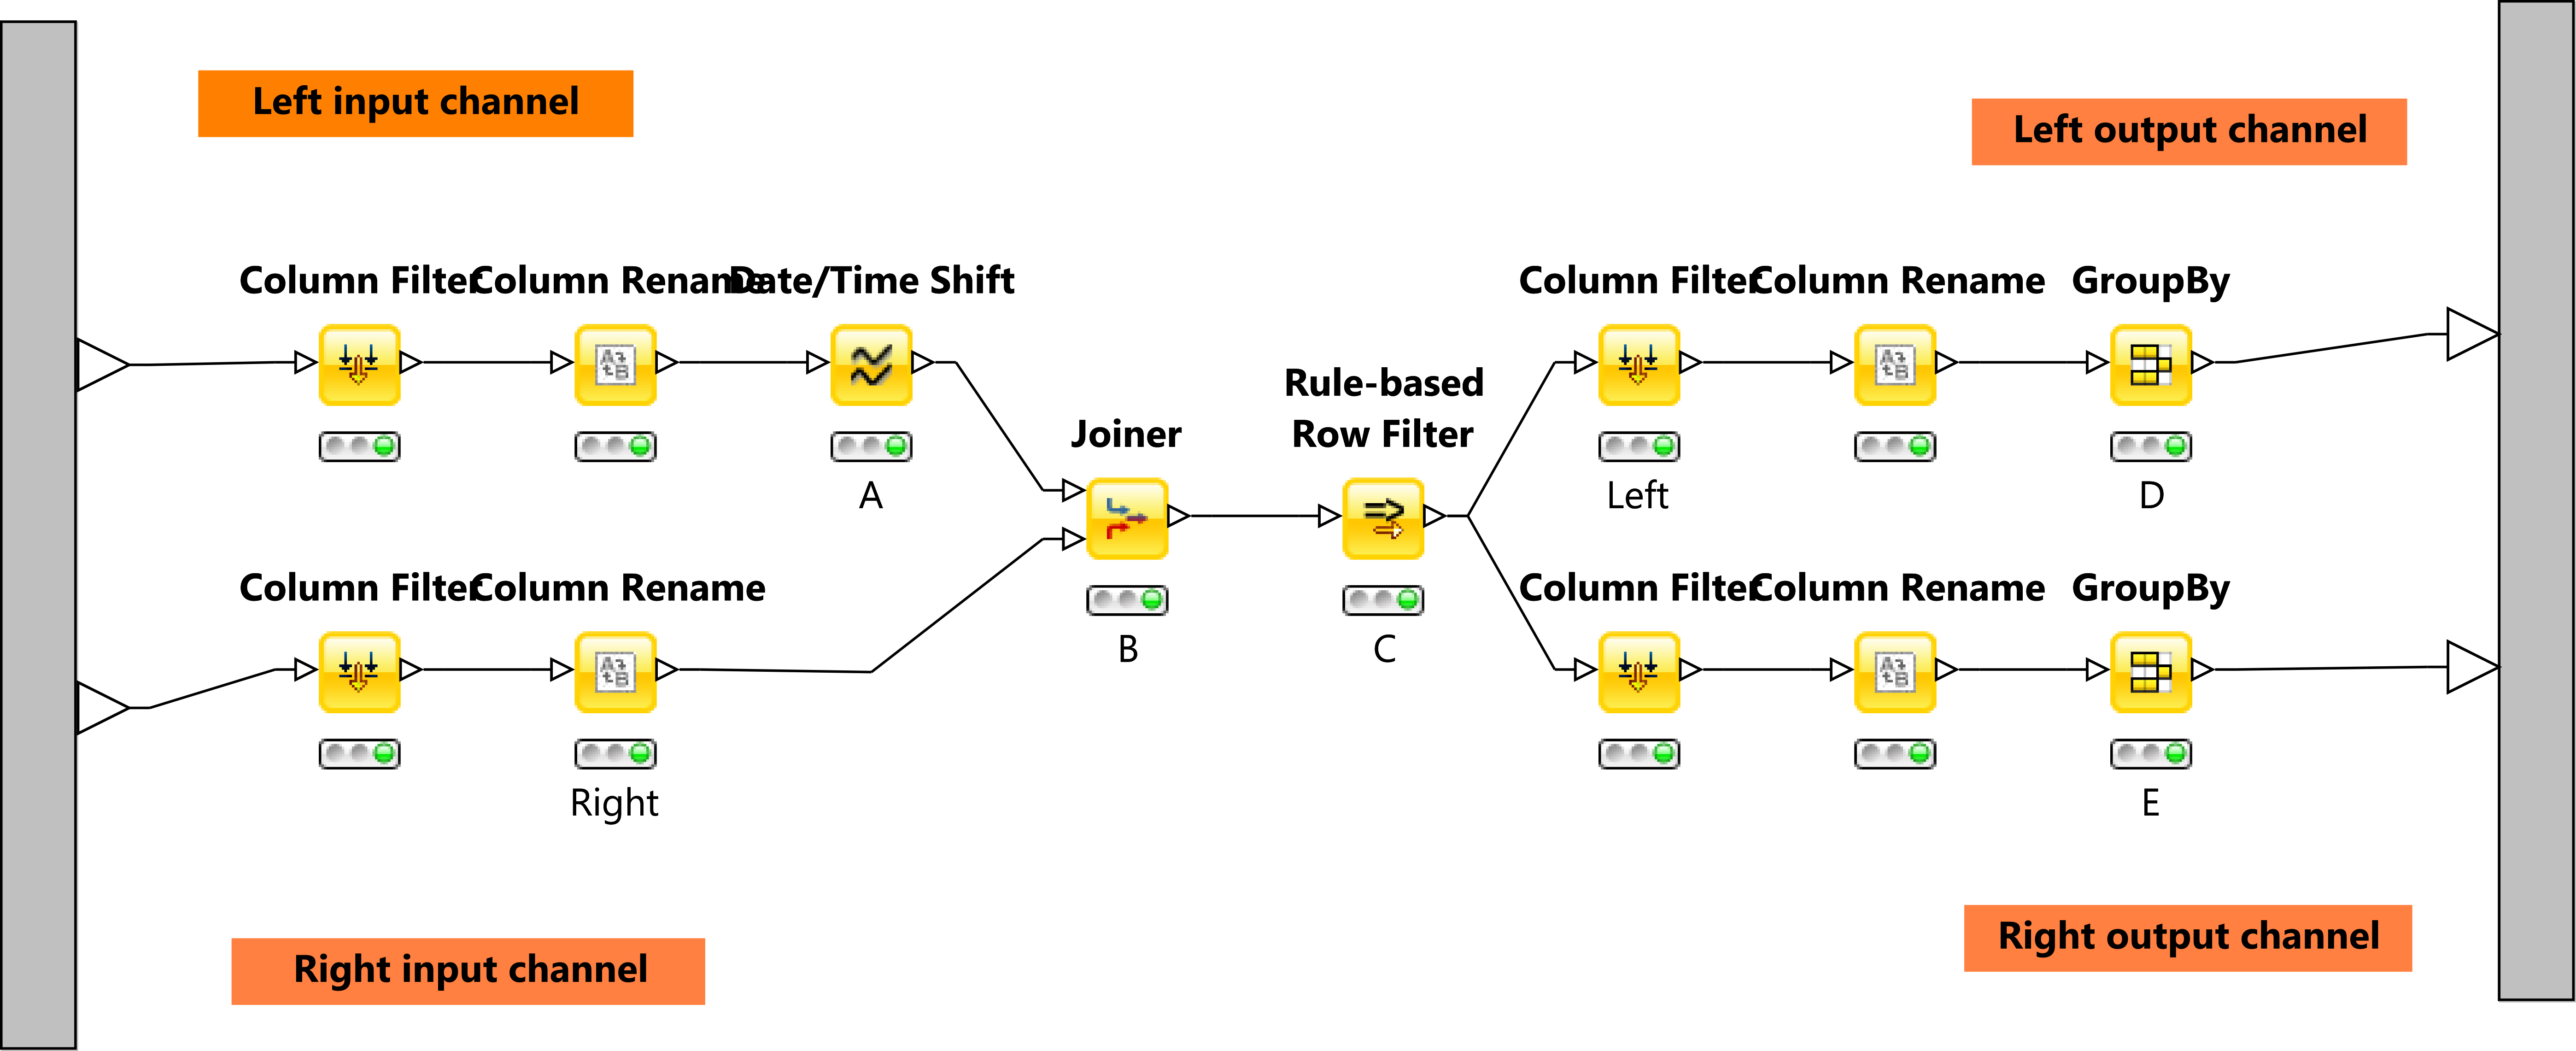
\includegraphics[width=0.8\textwidth]{figures/knime-snapshot-2.png}
	\caption{Implementing the temporal operator (\texttt{$\leq$ 30 day(s) starts before start of})}\label{fig:knime-snapshot-2}
\end{figure}
\vspace{5pt}

\textbf{Temporal Operators} (\texttt{$\leq$ 30 day(s) starts before start of}): This temporal operator (see Figure \ref{fig:knime-snapshot-2}) takes two input tables (denoted with \emph{left} and \emph{right}) each with at least two fields (\texttt{pid} and \texttt{StartDatetime}). First, we create a new column (called \texttt{LeftAdded}) on the left input table with 30 days added to their \texttt{StartDatetime} (Node A on Figure \ref{fig:knime-snapshot-2}). Then we inner join the left and right input tables with \texttt{pid} (Node B), and filter the rows where the \texttt{StartDatetime} (left) is earlier than \texttt{StartDatetime} (right) AND \texttt{LeftAdded} is not earlier than \texttt{StartDatetime} (right) (Node C). Then, we split the joined table back to the left and right output tables (corresponding to input tables) with removing duplicated rows (Node D and E). 

\textbf{Logical operators} (\texttt{AND}, \texttt{AND NOT}, \texttt{OR}): These are implemented with the operations shown in Table \ref{tab:boolean}.  For each instance of these operators, two customizations need to be addressed.  First, logical operators mostly use outputs from temporal operators, which have two output tables corresponding to their two input tables, so the logical operators need to select the semantically correct table to use.  Second, algorithms for logical operators require carefully selecting appropriate input columns in the joining steps, depending on whether they are operating on event-level data or patient-level data.  

\vspace{5pt}
\begin{table}[h]
\begin{center}
\begin{tabular}{p{0.2\textwidth}p{0.65\textwidth}}
\toprule
Operator	&Algorithm Steps \\
\midrule
\texttt{AND}	&\begin{enumerate} 
  \item Inner join two input tables using appropriate columns;
  \item Filter columns for the output table;
  \item Remove duplicated rows (with \texttt{GroupBy}).
\end{enumerate}
\\ 
\texttt{AND NOT}	&\begin{enumerate} 
  \item Add a column with non-null values to right-hand-side input table;
  \item Left outer join two input tables using appropriate columns;
  \item Filter and keep rows that have null in the added column from step 1;
  \item Filter columns for the output table and remove duplicated rows.
\end{enumerate}
\\ 
\texttt{OR}	&\begin{enumerate} 
  \item Filter appropriate columns from both input tables;
  \item Concatenate the two trimmed input tables and remove duplicated rows.
\end{enumerate}
\\ 
\bottomrule
\end{tabular}
\caption{Algorithms used in implementing QDM logical operators} 
\label{tab:boolean}
\end{center}
\end{table}

\subsection{Tested Dataset}

At VU, we tested this implementation with the Synthetic Derivative (SD) database\cite{roden_development_2008}, which contains de-identified clinical information derived from VU's EHR systems. The SD database contains clinical and demographic information, including as diagnosis codes, procedure codes, medications, laboratory values, and de-identified clinical documents and reports. It can be used as a stand-alone research resource, or in conjunction with BioVU to identify record sets for genome-phenome analysis. The execution was carried out on a desktop environment, so we used the subset of VU's genotyped population of 35,842 patients, with the measure period set at 2005-05-01 and ending at 2012-04-30.

At NU, we tested this implementation with data stored in the Northwestern Medicine Enterprise Data Warehouse (NMEDW) (\url{http://informatics.northwestern.edu/blog/edw}). The execution was also carried out on a desktop environment, so we used the subset of NU's genotyped population of 4,838 patients, with the same temporal period used for VU.  The NMEDW contains clinical and demographic data aggregated primarily from two commercial EHR systems (Cerner and Epic). It also contains basic information on research subjects, including those enrolled in NU's NUgene DNA biobank.


%-----------------------------------------------------------------------------
\section{Results and Discussion}
%-----------------------------------------------------------------------------

In developing this prototype, we address the current gap between the specification of QDM-based eCQMs and their application to existing clinical data. Continuing work on standardizing EHR systems is imperative to ensuring the efficacy of secondary use of future EHR data. At the same time, the currently available EHR data are an invaluable resource for the design and validation of QDM-based measures and algorithms.

In addition to enabling a QDM implementation, KNIME provides a very flexible platform with a full array of computational and programming tools for extending measures with downstream analysis (e.g., machine learning, statistics, graphical reports) that is not part of the QDM per se. It is also quite easy to adjust the connections between KNIME nodes and/or add additional nodes to provide further customization for end users. For example, CMS30 uses statins as discharge medication, and our final score for VU is only 35\%. However, if we use statins as ordered medication during the inpatient encounter, our score increases to 80\%. These two situations are virtually equivalent, and the discrepancy in scores arise mostly from variation in the documentation that we searched as part of this exercise -- excluding one of the most common discharge notes in the first analysis. (A score of 80\% is still lower than expected, perhaps due to specific exclusions, inclusion errors, or hospital transfers.) At NU, 85\% of the patients met the measure, when using medications ordered during inpatient stays, the closest surrogate to medications ordered at discharge. The score remained the same even when expanded to all ordered medications, including those ordered during outpatient encounters.

There are a few limitations to the work described here. First, the tools to automatically translate HQMF to KNIME or vice versa have not yet developed, so there is no current connection between QDM measures authored in MAT and those implemented in KNIME. Second, our current prototype implementation uses KNIME metanodes, which may be more difficult for users to adapt to new measures and local environments. We plan to develop a complete QDM extension package for KNIME to provide native QDM nodes for a better user experience. Third, data for some QDM Data Elements (e.g., medication order not done) and attributes (e.g., discharge status) are not readily available in either VU or NU integrated data marts, and their implementation in KNIME requires future work. Fourth, we do not eliminate the need for informaticians with basic skills in SQL and programming to author and adapt measures and algorithms. Instead, our goal for this project is to enable these informaticians to use the QDM with their own projects, and to share executable artifacts with external institutions. Enabling of such a user community is important for the evolution and adoption of the QDM.

%-----------------------------------------------------------------------------
\section{Acknowledgements}
%-----------------------------------------------------------------------------

This work has been supported in part by funding from PhEMA (R01 GM105688) and eMERGE (U01 HG006379, U01 HG006378 and U01 HG006388).

\centering
\bibliographystyle{vancouver}
\bibliography{2015-AMIA-CRI}


\end{document}
